% This file is the basic running of the model, just the population growth of Kiribati


\section{Demographics}
\subsection{Crude birth rate and death rate}
Births are modelled using time-variant crude birth rates that are multiplied by the modelled population 
size to determine the number of newborn individuals entering the youngest age category (0 - 4) at each time. A time-variant 
and age-specific rate of non-TB-related mortality applies to all model compartments to simulate 
deaths from other causes than TB. We use estimates from the UN Population Division\footnote{https://population.un.org/wpp/Download/Standard/Mortality/} to inform the 
birth and mortality rates.
We also apply additional death rates to the compartment I to reflect mortality induced by TB 
disease.
\begin{table}[!htp]
    \caption{\textbf{Model Parameters}}
    \label{tab:parameter}
    \begin{threeparttable}
    \begin{tabularx}{\textwidth}{ X  X  X }
        \hline
        \textbf{Parameter} & \textbf{Value} & \textbf{Source} \\
        \hline
        \textbf{Population characteristics} & & \\
        
ISO3 code for source country for mixing matrix & GBR  & Closest demographic profile to Australia \\ 
\hline
Starting infectious seed & 2.0 persons & Arbitrary \\ 
\hline
Proportion of active period before isolation & 0.333  & Assumed \\ 
\hline
Relative infectiousness of asymptomatic persons per unit time & 0.5  & Assumed \\ 
\hline
Relative infectiousness of isolated cases & 0.2  & Assumed \\ 
\hline
Reduction in transmission risk for boosted & 0.6  & Viral load substantially lower in boosted compared to two dose vaccinated persons \cite{puhach-2022} \\ 
\hline
Reduction in transmission risk for primary course & 0.2  & Half of estimate of 40\% for Delta \cite{eyre-2022, harris-2021} \\ 
\hline
Adjustment to base case fatality rates & 0.15  & Adapted to match local epidemiology \\ 
\hline
BA.1 infection cross protection against BA.5 infection & 0.0  & No immunity from BA.1 is retained through to the BA.5 period \\ 
\hline
BA.2 infection cross protection against BA.1 infection & 1.0  & Immunity from subsequent strains is assumed to completely protect against previous strains \\ 
\hline
BA.5 infection cross protection against BA.1 infection & 1.0  & Immunity from subsequent strains is assumed to completely protect against previous strains \\ 
\hline
BA.5 infection cross protection against BA.2 infection & 1.0  & Immunity from subsequent strains is assumed to completely protect against previous strains \\
        Crude birth rate  & Time-variant & UN Population Divison \\
        Universal death rate & Time-variant & UN Population Divison \\
        \hline
        \textbf{\emph{M.tb} infection and TB} \\
        Rate of stabilization from early to late latency (age 0-4/5-14/15+) & 4.4/4.4/2 per year & Ragonnet et al.\cite{ragonnet-2022} \\
        Rate of rapid progression to active TB (age 0-4/5-14/15+) & 2.4/2/0.1 per year & Ragonnet et al.\cite{ragonnet-2022} \\
        Rate of late reactivation (age 0-4/5-14/15+) & 7e\textsuperscript{-9}/2.3e\textsuperscript{-3}/1.2e\textsuperscript{-3} per year & Ragonnet et al.\cite{ragonnet-2022} \\
        Relative risk of reinfection while latently infected (ref. infection-naive) & 0.2 & Ragonnet et al.\cite{ragonnet-2022} \\
        Relative risk of reinfection after recovery (ref. infection-naive) & 0.2 & Ragonnet et al.\cite{ragonnet-2022} \\
        \hline
	\end{tabularx}
    \end{threeparttable}
\end{table}
1
\begin{figure}[!htp]
   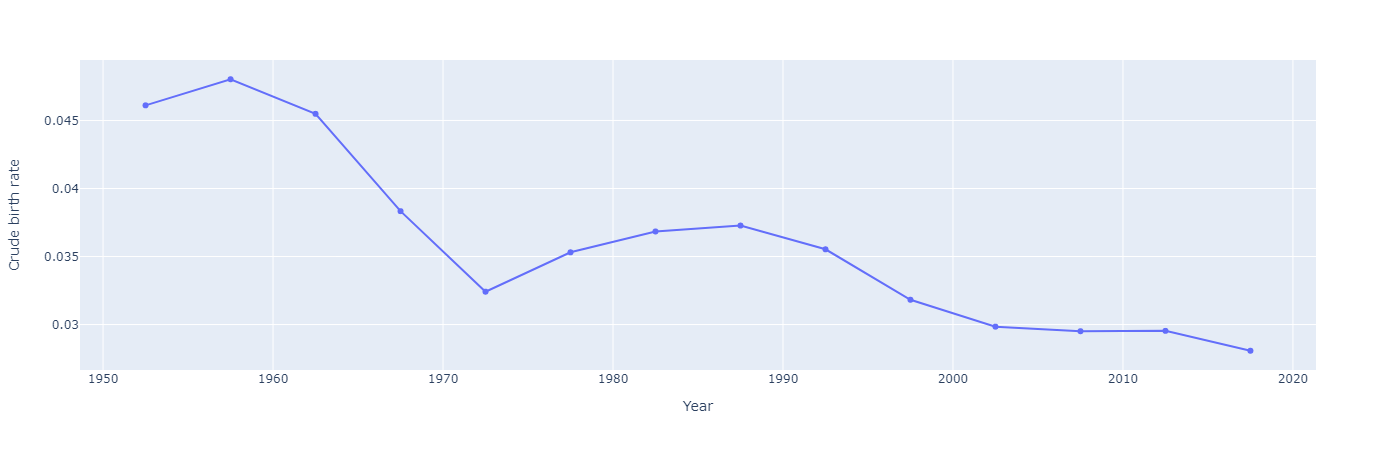
\includegraphics[width=\textwidth,keepaspectratio]{images/cbr.png}
    \caption{The crude birth rate of Kiribati from 1950 to 2020.}
    \label{fig:cbr}
\end{figure}

\begin{figure}[!htp]
   \centerline{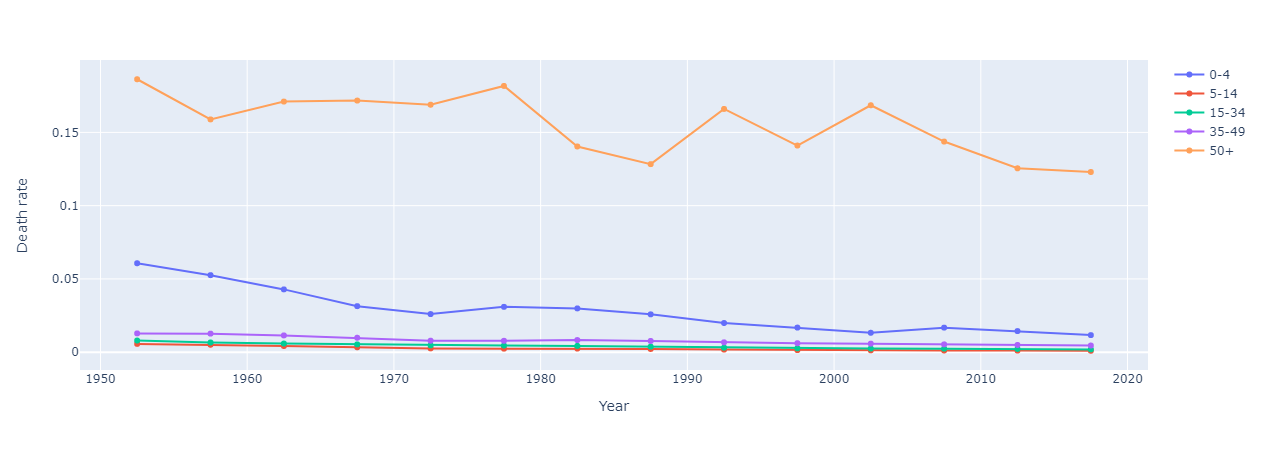
\includegraphics[width=\textwidth,keepaspectratio]{images/cdr.png}}
    \caption{The death rate of Kiribati from 1950 to 2020, stratified by age group.}
    \label{fig:cdr}
\end{figure}

\subsection{Comparing modelled population with actual population}
\begin{figure}[!htp]
    \centerline{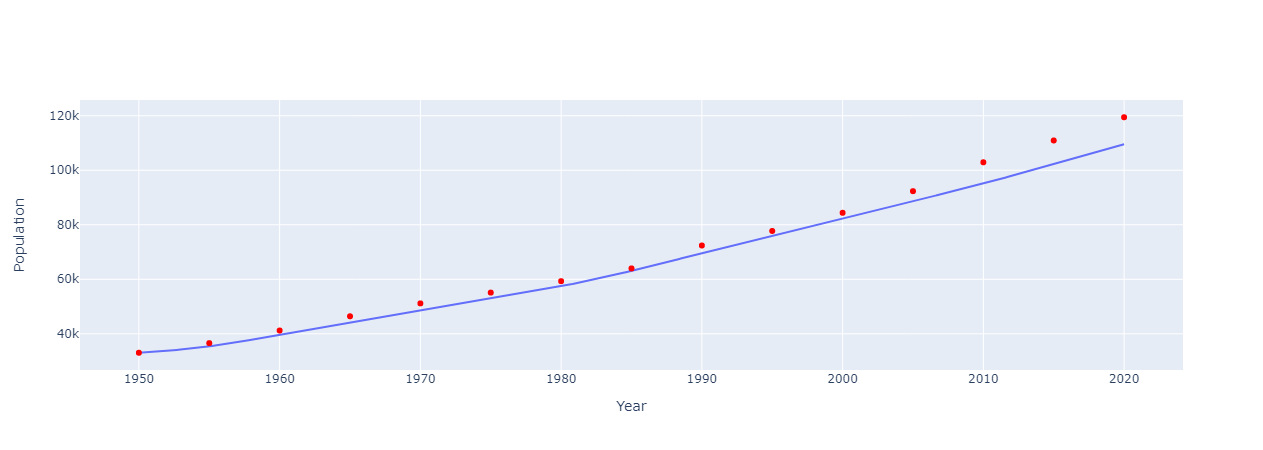
\includegraphics[width=\textwidth,keepaspectratio]{images/modelled_total.png}}
    \caption{Comparing modelled population with actual population of Kirbati from 1950 to 2020. The red dots represent the actual population size of Kiribati,
     while the blue line represents the modelled population size}
    \label{fig:modelled_total}
\end{figure}

\begin{figure}[htp]
    \centerline{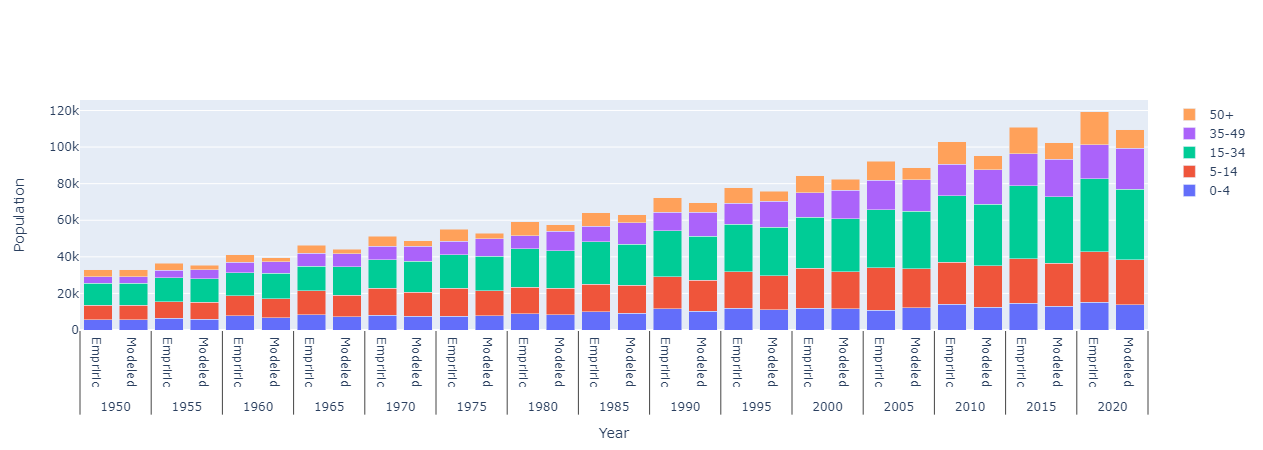
\includegraphics[width=\textwidth,keepaspectratio]{images/compare_pop.png}}
    \caption{Comparing modelled population with actual population by age groups of Kirbati from 1950 to 2020.}
    \label{fig:compare_group}
\end{figure}